% Copyright 2025 Diego Correa Tristain <algoritmia@labormedia.cl>
%
% Permission is hereby granted, free of charge, to any person obtaining a
% copy of this document and associated documentation files (the "Document"),
% to deal in the Document without restriction, including without limitation
% the rights to use, copy, modify, merge, publish, distribute, sublicense,
% and/or sell copies of the Document, and to permit persons to whom the
% Software is furnished to do so, subject to the following conditions:

% The above copyright notice and this permission notice shall be included in
% all copies or substantial portions of the Document.
%
% THE DOCUMENT IS PROVIDED "AS IS", WITHOUT WARRANTY OF ANY KIND, EXPRESS
% OR IMPLIED, INCLUDING BUT NOT LIMITED TO THE WARRANTIES OF MERCHANTABILITY,
% FITNESS FOR A PARTICULAR PURPOSE AND NONINFRINGEMENT. IN NO EVENT SHALL THE
% AUTHORS OR COPYRIGHT HOLDERS BE LIABLE FOR ANY CLAIM, DAMAGES OR OTHER
% LIABILITY, WHETHER IN AN ACTION OF CONTRACT, TORT OR OTHERWISE, ARISING
% FROM, OUT OF OR IN CONNECTION WITH THE SOFTWARE OR THE USE OR OTHER
% DEALINGS IN THE SOFTWARE.

%Graphical representation of a grid by:
%Author: Marco Miani
%Resoure: https://www.tudelft.nl/citg/over-faculteit/afdelingen/hydraulic-engineering/sections/environmental-fluid-mechanics/research/swan
%SWAN (developed by SWAN group, TU Delft, The Netherlands) is a wave spectral numerical model.
%For Simlating WAves Nearshore, it is necessary to define spatial grids of
%physical dominant factors (wind friction, dissipation) as well as define a COMPUTATIONAL
%grid on which the model performs its (spectral) calculations: budgeting energy spectra over
%each cell of the (computational) grid. Grids might have different spatial resolution and extension.

\documentclass[12pt]{article}
\usepackage{algorithm}
\usepackage{algpseudocode}
\usepackage{amsmath}
\usepackage{amssymb}
\usepackage{tikz}
\usetikzlibrary{positioning}

\title{Emergent Properties of Distributed Agents with Two-Stage Convex Zero-Sum Optimal Exchange Network}
\author{Diego Correa Tristain \\ \texttt{algoritmia@labormedia.cl}}

\begin{document}
\pagestyle{empty}

\maketitle

\section{Introduction}
This paper examines network behaviour of distributed systems under the assumptions of optimal convex programming zero-sum transitions for a two step evaluation network of agents, with stages consisting of: \newline
a) An evaluation of the best exchange outcome for each agent within its neighborhood, \newline
b) The execution of optimal matching pairs driven by the first stage evaluation.\\
Each agent has access to the evaluation of its immediate neighborhood within a lattice of indices $\{(i, j) \mid 1 \leq i \leq n, \ 1 \leq j \leq m\}$ with canonical base [(1,0), (0,1)] and continuous space of size \(n \times m\), where $C_{i, j+1}$ is considered as part of the neighborhood for agent $C_{i, j}$, and $j + 1 \equiv (j + 1)\ mod\ \max_k$, with $\max_k$ being the maximum number of agents for that row or column in the lattice order.

\section{Problem Setting}
Let \(G_{t}\) be a two-dimensional lattice \(G\) for time \(t\) with size \(n \times m\). The state of \(G_{t}\) is the collected states of all individual states \(s_{i,j}(t) \in \mathbb{R}^2\) of each cell \(C_{i,j}\) (where \(i, j\) are row and column indices) at time \(t\).
  
Let \(N_{i,j}\) be the neighborhood of a cell \(C_{i,j}\), i.e. the set of cells that influence its state. For example, in Von Neumann neighborhood:

  \[
  N_{i,j} = \{C_{i-1,j}, C_{i+1,j}, C_{i,j-1}, C_{i,j+1}\} \tag{2.1}% Moore's , C_{i-1,j-1}, C_{i-1,j+1}, C_{i+1,j-1}, C_{i+1,j+1}
  \] 
  
     \begin{center}
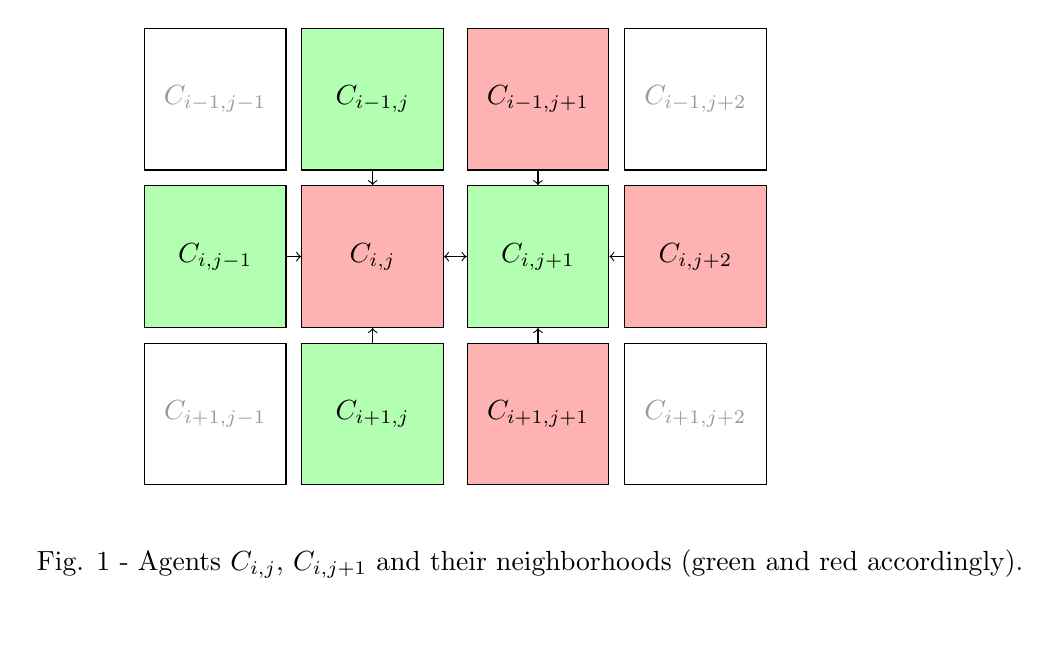
\begin{tikzpicture}[scale=2, every node/.style={rectangle, draw, minimum size=1.8cm}]

    % First agent
    \node (A)[fill=green, fill opacity=0.3, text=black, text opacity=1]  at (-1, 2) {$C_{i-1,j}$};
    
    \node (B)[fill=green, fill opacity=0.3, text=black, text opacity=1] at (-2, 1) {$C_{i,j-1}$};
    \node (C)[fill=red, fill opacity=0.3, text=black, text opacity=1]  at (-1, 1) {$C_{i,j}$}; % Central cell
    %\node (D) at (1, 1) {$C_{i,j+1}$};

    \node (H)[fill=green, fill opacity=0.3, text=black, text opacity=1] at (-1, 0) {$C_{i+1,j}$};
    
    % Draw edges to represent interdependencies (Von Neumann neighborhood)

    
    % Second agent
    \node (E)[fill=red, fill opacity=0.3, text=black, text opacity=1] at (0.05, 2) {$C_{i-1,j+1}$};
    
    %\node (F) at (0, 1) {$C_{i,j-1}$};
    \node (G)[fill=green, fill opacity=0.3, text=black, text opacity=1] at (0.05, 1) {$C_{i,j+1}$}; % Central cell
    \node (O)[fill=red, fill opacity=0.3, text=black, text opacity=1]  at (1.05, 1) {$C_{i,j+2}$};

    \node (P)[fill=red, fill opacity=0.3, text=black, text opacity=1]  at (0.05, 0) {$C_{i+1,j+1}$};
    
    \node (Z1)[fill=white,fill opacity=.4] at (-2, 2) {$C_{i-1, j-1}$};
    \node (Z1)[fill=white,fill opacity=.4] at (-2, 0) {$C_{i+1, j-1}$};
    \node (Z1)[fill=white,fill opacity=.4] at (1.05, 2) {$C_{i-1, j+2}$};
    \node (Z1)[fill=white,fill opacity=.4] at (1.05, 0) {$C_{i+1, j+2}$};
    
    % Edges for c_{i,j}
    \draw[->] (A) -- (C);
    \draw[->] (B) -- (C);
    \draw[->] (G) -- (C);
    \draw[->] (H) -- (C);
    
    % Draw edges to represent interdependencies (Von Neumann neighborhood)
    \draw[->] (E) -- (G);
    \draw[->] (C) -- (G);
    \draw[->] (O) -- (G);
    \draw[->] (P) -- (G);
    \begin{scope}[shift={(0, -0.5)}]  
        \node[below, rectangle, draw=none] {Fig. 1 - Agents ${C_{i,j}}$, ${C_{i,j+1}}$ and their neighborhoods (green and red accordingly). };
    \end{scope}
\end{tikzpicture}
\end{center}

Let \(\mathbf{P}_{i,j} \in \mathbb{R}^2\) be the parameters associated with agent \(C_{i,j}\).
  
 \section{First Stage: Optimal Evaluation Function}
 
   \subsection{Peer to Peer Convex Programming Evaluation}
  
  Let function \( o_{\mathbf{P}_{i,j}}: \mathbb{R}^2 \to \mathbb{R} \) be a \textit{strictly convex function} with constant parameters \(\mathbf{P}_{i,j}\) such that for all \( x_1, x_2 \in \mathbb{R}^2 \) and for all \( \lambda \in [0, 1] \):

\[
o_{\mathbf{P}_{i,j}}(\lambda x_1 + (1 - \lambda) x_2) < \lambda o_{\mathbf{P}_{i,j}}(x_1) + (1 - \lambda) o_{\mathbf{P}_{i,j}}(x_2) \tag{3.1.1}
\]

Let \(o_{\mathbf{P}_{i,j}}\) be also \textit{strictly monotonically increasing}:

\[
\forall x_1, x_2 \in \mathbb{R}^2 
\]
\[
|x_1| < |x_2| 
\iff o_{\mathbf{P}_{i,j}}(x_1) < o_{\mathbf{P}_{i,j}}(x_2) \tag{3.1.2}
\]

 \subsection{Objective Function}
 
 Let's $O_{i,j}$ be the objective function for cell $C_{i,j}$ that depends on parameters $\mathbf{P}_{i,j} \in \mathbb{R}^{2}$, it's own current state $s_{i,j}(t)$ and the parameters with the current states of its neighbors. The result registers the neighbor cell that yields the best outcome for its objective function and its associate state transition, the exchange vector \(\vec{e}_{i,j} \in \mathbb{R}^{2}\):
  \[
  O_{i,j}(t+1) = \mathcal{L}\left(\mathbf{P}_{i,j},s_{i,j}(t), \{\mathbf{P}_{k,l},s_{k,l}(t) \mid \forall C_{k,l} \in N_{i,j}\}\right)
  \]
  \[
  = \{\vec{e}_{(i,j) (r,q)} \in \mathbb{R}^{2} \mid C_{r,q} \in N_{i,j}\}\tag{3.2.1}
  \]
  
  A necessary condition of this model is that every optimal evaluation participates of a zero-sum game associated with their optimal exchanges, i.e:\\
  \[
  \forall (i, j), (r,q) \mid i,r \in \{1, \dots, n\}; \ j, q \in \{1, \dots, m\}
  \]
  \[
  O_{i,j}(t+1) = \{\vec{e}_{(i,j) (r,q)} \mid C_{r,q}\}
  \]
  \[
  \land \ O_{r,q}(t+1) = \{\vec{e}_{(r,q) (i,j)} \mid C_{i,j}\}
  \]
  \[
    \implies \vec{e}_{(i,j) (r,q)} + \vec{e}_{(r,q) (i,j)} = \vec{0} \tag{3.2.2}
  \]
  \[
    \implies \vec{e}_{(i,j) (r,q)} = - \vec{e}_{(r,q) (i,j)} \tag{3.2.3}
  \]
  
  As, by definition, optimal matching pairs are evaluated from their neighborhoods, this pair lies in the intersection of their neighborhoods:
  
    \[
  \forall \ C_{i, j} \in N_{r,q}, \forall C_{r,q} \in N_{i,j} 
  \]
  \[
  O_{i,j}(t+1) = \{\vec{e}_{(i,j) (r,q)} \mid C_{r,q}\}
  \]
  \[
  \land \ O_{r,q}(t+1) = \{\vec{e}_{(r,q) (i,j)} \mid C_{i,j}\}
  \]
  \[
    \implies \vec{e}_{(i,j) (r,q)} = - \vec{e}_{(r,q) (i,j)} \tag{3.2.4}
  \]
  
  In this way, the optimal matches of agents can be calculated locally within their neighborhoods by:
  
    \[
  O_{i,j}(t+1) = \text{maximize} \quad \mathcal{L}\left(\mathbf{P}_{i,j},s_{i,j}(t), \{\mathbf{P}_{k,l},s_{k,l}(t) \mid \forall C_{k,l} \in N_{i,j}\}\right)
  \]
  \[
  = \max_{\vec{v} \in \mathbb{R}^{2}} \{ \text{maximize} \quad o_{\mathbf{P}_{i,j}}(\vec{v}) \quad  \text{subject to}
  \]
  \[
  \quad \vec{v}_{(i,j)(k,l)} + \vec{u}_{(k,l)(i,j)} = \vec{0}  \quad \text{for} \quad \{o_{\mathbf{P}_{k,l}}(\vec{u}) \mid \forall C_{k,l} \in N_{i,j}\} \}
  \]
  \[
  = \{\vec{e}_{(i,j) (r,q)} \in \mathbb{R}^{2} \mid C_{r,q} \in N_{i,j}\} \tag{3.2.5}
  \]
  
  This is, the vector \(\vec{e}_{(i,j) (r,q)}\) in all the vectors \(\vec{v} = \vec{e}_{(i,j) (r,q)}\) and \(\vec{u} = \vec{e}_{(r,q) (i,j)} = -\vec{e}_{(i,j) (r,q)}  ,\quad \forall C_{r,q} \in N_{i,j} \), that yields the maximum value to the peer to peer convex programming evaluation.

\subsection{Uniqueness of Optimal Pair Evaluations}

Appendix A provides a demonstration for the uniqueness of the optimal pair:

    \[
  \forall \ C_{i, j} \in N_{r,q}, \forall C_{r,q} \in N_{i,j} 
  \]
  \[
  O_{i,j}(t+1) = \{\vec{e}_{(i,j) (r,q)} \mid C_{r,q}\}
  \]
  \[
  \land \ O_{r,q}(t+1) = \{\vec{e}_{(r,q) (i,j)} \mid C_{i,j}\}
  \]
  \[
    \iff \exists! \vec{e}_{(i,j) (r,q)} \in \mathbb{R}^2, 
  \]
  \[
  \exists! \vec{e}_{(r,q) (i,j)} \in \mathbb{R}^2
  \]
  \[
    \vec{e}_{(i,j) (r,q)} + \vec{e}_{(r,q) (i,j)} = \vec{0} \tag{3.3.1}
  \]
  

\section{Second Stage: Grid State Transition}

\subsection{Agent State Update}

The state of each agent at the next time step is defined by its objective function such that:

  \[
    O_{i,j}(t+1) = \{\vec{e}_{(i,j) (r,q)} \mid C_{r,q}\}
  \]
  \[
  \land \ O_{r,q}(t+1) = \{\vec{e}_{(r,q) (i,j)} \mid C_{i,j}\}
  \]
  \[
  \iff s_{i,j}(t+1) = s_{i,j}(t) + \vec{e}_{(i,j) (r,q)}
  \]
  \[
  \land \ s_{r,q}(t+1) = s_{r,q}(t) + \vec{e}_{(r,q) (i,j)} \tag{4.1.1}
  \]
  
These are the only state transitions that $C_{i,j}$ and $C_{r,q}$ will execute in update $G_{t+1}$, all others discarded, for all pairs of optimal transactions in their respective neighborhoods.

\begin{center}
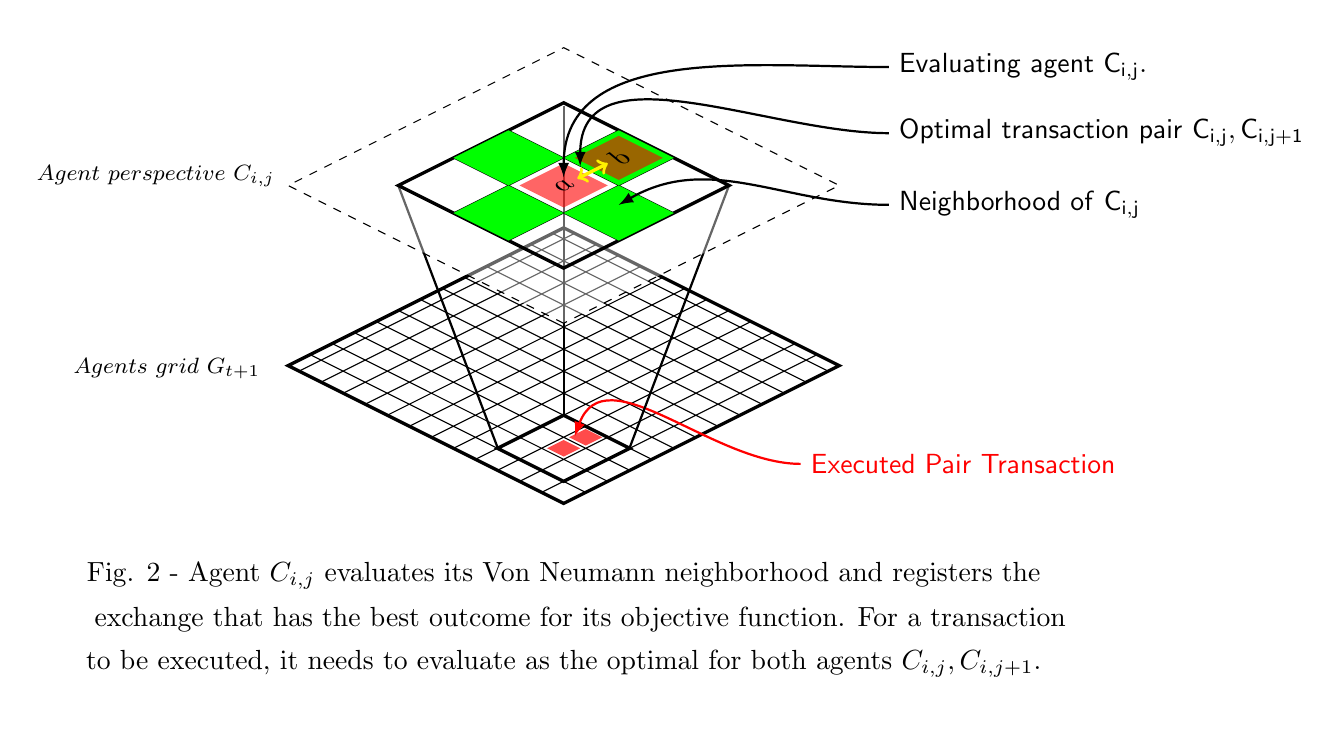
\begin{tikzpicture}[scale=.7,every node/.style={minimum size=1cm},on grid]
		
    %slanting: production of a set of n 'laminae' to be piled up. N=number of grids.
    \begin{scope}[
            yshift=-83,every node/.append style={
            yslant=0.5,xslant=-1},yslant=0.5,xslant=-1
            ]
        % opacity to prevent graphical interference
        \fill[white,fill opacity=0.5] (0,0) rectangle (5,5);
        \draw[step=4mm, black] (0,0) grid (5,5); %defining grids
        \draw[black,very thick] (0.4,0.4) rectangle (1.6,1.6);
        %\draw[step=1mm, red!50,thin] (3,1) grid (4,2);  %Nested Grid
        \draw[black,very thick] (0,0) rectangle (5,5);%marking borders
        \fill[red, fill opacity=0.7] (0.85,0.85) rectangle (1.15,1.15); % cells advances every 0.4 points
        \fill[red, fill opacity=0.7] (1.25,0.85) rectangle (1.55,1.15);
        %Idem as above, for the n-th grid:
    \end{scope}
    
    %\draw[-latex,thick,red](4.3,-1.9)node[right]{$\mathsf{Nested\ G.}$}
     %   to[out=180,in=90] (2,-.5);
    
    \draw[-latex,thick,red](4.3,-2.2)node[right]{$\mathsf{Executed\ Pair\ Transaction}$}
        to[out=180,in=70] (0.2,-1.7);
    	
    %\begin{scope}[
    	%yshift=0,every node/.append style={
    	%    yslant=0.5,xslant=-1},yslant=0.5,xslant=-1
    	             ]
        %\fill[white,fill opacity=.9] (0,0) rectangle (5,5);
        %\draw[black,very thick] (0,0) rectangle (5,5);
        %\draw[step=5mm, black] (0,0) grid (5,5);
    %\end{scope}
     \draw[thick] (-3,2.85) -- (-1.2,-1.9);
     \draw[thick] (3,2.85) -- (1.2,-1.9);
     \draw[thick] (0,4.3) -- (0,-1.3);
    	
    \begin{scope}[
    	yshift=10,every node/.append style={
    	yslant=0.5,xslant=-1},yslant=0.5,xslant=-1
    	             ]
    	\fill[white,fill opacity=.4] (0,0) rectangle (5,5);
    	\draw[step=10mm, black] (1,1) grid (4,4);
    	\draw[black,very thick] (1,1) rectangle (4,4);
    	\draw[black,dashed] (0,0) rectangle (5,5);
	\fill[green] (2,1) rectangle (3,2);
	\fill[green] (2,2) rectangle (1,3);
	\fill[green] (2,3) rectangle (3,4);
	\fill[green] (4,2) rectangle (3,3);
	\fill[red, fill opacity=0.6] (2.9,2.1) rectangle (2.1,2.9);
	\fill[red, fill opacity=0.6] (3.9,2.1) rectangle (3.1,2.9);
	\draw[<->,yellow, very thick] (3.3,2.5) -- (2.75,2.5);
	\draw[](2.5,2.5)node{${a}$};
	\draw[](3.5,2.5)node{${b}$};
    \end{scope}
    \fill[black,font=\footnotesize]
        (-7.2,-1.2) node [above] {$Agents\ grid\ G_{t+1}$};
        
    \fill[black,font=\footnotesize]
        (-7.4, 2.3) node [above] {$Agent\ perspective\ C_{i,j}$};

    \draw[-latex,thick](5.9,2.5)node[right]{$\mathsf{Neighborhood\ of\ {C_{i,j}}}$}
        to[out=180,in=30] (1,2.5);
    \draw[-latex,thick](5.9,5.0)node[right]{$\mathsf{Evaluating\ agent\ {C_{i,j}}.}$}
        to[out=180,in=90] (0,3.0);
    \draw[-latex,thick](5.9,3.8)node[right]{$\mathsf{Optimal\ transaction\ pair\ {C_{i,j}, C_{i, j+1}}}$}
        to[out=180,in=90] (0.3,3.2);
    
    % Footer
    \begin{scope}[shift={(0, -3.5)}]  
        \node[below] {Fig. 2 - Agent ${C_{i,j}}$ evaluates its Von Neumann neighborhood and registers the };
        \node[below] at (0.3,-0.8) {exchange that has the best outcome for its objective function. For a transaction};
        \node[below] at (-0.0,-1.6) {to be executed, it needs to evaluate as the optimal for both agents $C_{i,j}, C_{i, j+1}$.};
    \end{scope}

\end{tikzpicture}
\end{center}

\section{Algorithm and Simulation Procedure}

\begin{algorithm}
\caption{Distributed Convex Optimization for Multiple Agents}
\begin{algorithmic}[1]
\State Initialize agent parameters \( \mathbf{P}_{i,j}^0 \) and state \( s_{i,j}^0\)for all agents $\{(i, j) \mid 1 \leq i \leq n, \ 1 \leq j \leq m\}$ in grid $G_{0}^{n \times m}$.
\State Initialize registers \( \textbf{S1}^{n \times m} \) and \( \textbf{S2} \)
\For{each iteration \( t = 0, 1, \dots, T \)}
    \State Initialize a new grid \( G_{t+1} \) of the same size as \( G_{t} \)
    \For{each agent \( C_{i,j} \)}
        \State Get neighborhood \( N_{i, j} \) of agent \( C_{i, j} \)
        \For {each agent \(C_{k,l}\) in \(N_{i,j}\)}
            \State Get parameters \( \mathbf{P}_{k,l} \)
            \State  solve the local optimization problem:
            \[
            \mathbf{\vec{e}}_{(i,j)(k,l)}^{t+1} = \arg \max_{\mathbf{\vec{e}}_{(i,j)(k,l)}} \left( o_{\mathbf{P}_{i,j} }(\vec{e}_{(i,j)(k,l)}) + \lambda_{(i,j)(k,l)} \left( \vec{e}_{(i,j)(k,l)} + \vec{e}_{(k,l)(i,j)} \right) \right)
            \]
            where \( \lambda_{(i,j)(k,l)} \) is the dual variable associated with the coupling constraint and \( \vec{e}_{(k,l)(i,j)} \) is the optimal dual solution from the perspective of agent \( C_{k,l} \), this is:
            \[
            \mathbf{\vec{e}}_{(k,l)(i,j)}^{t+1} = \arg \max_{\mathbf{\vec{e}}_{ki,l)(i,j)}} \left( o_{\mathbf{P}_{k,l} }(\vec{e}_{(k,l)(i,j)}) + \lambda_{(k,l)(i,j)} \left( \vec{e}_{(k,l)(i,j)} + \vec{e}_{(i,j)(k,l)} \right) \right)
            \]
            
            where, by the constraint given:
            
            \[
            \mathbf{\vec{e}}_{(i,j)(k,l)}^{t+1} + \mathbf{\vec{e}}_{(k,l)(i,j)}^{t+1} = \vec{0}
            \]
            \State register solution \(\{ \mathbf{\vec{e}}_{(i,j)(k,l)}^{t+1} \mid C_{k,l} \in N_{i,j}  \}\) in \( \textbf{S1}^{n \times m} \)
        \EndFor
        \State Obtain \( O_{i,j}(t+1) = \max_{\mathbf{\vec{e}}_{(i,j)(k,l)}^{t+1}} \{ \mathbf{\vec{e}}_{(i,j)(k,l)}^{t+1} \mid C_{k,l} \in N_{i,j}  \} \in \textbf{S1}^{n \times m} \quad \)
        \If{\( \exists O_{k,l}(t+1) \in \textbf{S1}^{n \times m} \land O_{k,l} = \{ \mathbf{\vec{e}}_{(k,l)(i,j)}^{t+1} \mid C_{i,j} \in N_{k,l}  \}\)}
        % Write If condition for second stage.
            \State Register \( (O_{i,j}(t+1), O_{k,l}(t+1) )\) in \textbf{S2}
        \EndIf
    \EndFor
    \For{ \((O_{i,j}(t+1), O_{k,l}(t+1) ) \in \textbf{S2}\)} 
        \State Update agent states \( s_{i,j}^{t+1}, s_{k,l}^{t+1} \) adding the exchange vector to the previous state:
    \[
    s_{i,j}^{t+1} = s_{i,j}^{t} + \mathbf{\vec{e}}_{(i,j)(k,l)}^{t+1} 
    \]
    \[
    s_{k,l}^{t+1} = s_{i,j}^{t} + \mathbf{\vec{e}}_{(k,l)(i,j)}^{t+1} 
    \]
    \EndFor
\EndFor
\end{algorithmic}
\end{algorithm}

\newpage

\appendix
\section{Appendix: Uniqueness of Optimal Pair Evaluations}

This appendix provides detailed mathematical demonstration of the theorem stated in section 3.3 "Uniqueness of Optimal Pair Evaluations".

\subsection{Uniqueness of the Peer to Peer Convex Programming Evaluation}

Let \(o_{\mathbf{P}_{i,j}}(\vec{v})\) be the objective function for the convex programming evaluation:

\[
  \text{maximize} \quad o_{\mathbf{P}_{i,j}}(\vec{v}) \quad  \text{subject to}   \quad \vec{v}_{(i,j)(k,l)} + \vec{u}_{(k,l)(i,j)} = 0 \tag{A.1.1}
  \]
  \[
\text{for} \quad \{o_{\mathbf{P}_{k,l}}(\vec{u}) \mid \forall C_{k,l} \in N_{i,j}\} 
  \]
  
  Let \( \vec{e}_{(i,j) (r,q)} \) and \(\vec{e}_{(i,j) (r',q')}  \) be solutions for the \textit{strictly convex programming evaluation} for the  \( ( C_{i,j} , C_{r,q} )\) pair of agents. This is:

  \[
  o_{\mathbf{P}_{k,l}}(\vec{e}_{(i,j) (r,q)}) \geq o_{\mathbf{P}_{k,l}}(\vec{u}) \quad \text{for} \quad \{o_{\mathbf{P}_{k,l}}(\vec{u}) \mid \forall C_{k,l} \in N_{i,j}\} 
  \]  
    \[
  \land \quad o_{\mathbf{P}_{k,l}}(\vec{e}_{(i,j) (r',q')}) \geq o_{\mathbf{P}_{k,l}}(\vec{u}) \quad \text{for} \quad \{o_{\mathbf{P}_{k,l}}(\vec{u}) \mid \forall C_{k,l} \in N_{i,j}\} \tag{A.1.2}
  \]  
  \[
  \implies o_{\mathbf{P}_{k,l}}(\vec{e}_{(i,j) (r,q)}) \geq o_{\mathbf{P}_{k,l}}(\vec{e}_{(i,j) (r',q')})
  \]
    \[
  \land \quad o_{\mathbf{P}_{k,l}}(\vec{e}_{(i,j) (r,q)}) \leq o_{\mathbf{P}_{k,l}}(\vec{e}_{(i,j) (r',q')}) \tag{A.1.3}
  \]
    \[
  \implies o_{\mathbf{P}_{k,l}}(\vec{e}_{(i,j) (r,q)}) = o_{\mathbf{P}_{k,l}}(\vec{e}_{(i,j) (r',q')}) \tag{A.1.4}
  \]
  
  Let :
  
  \[ z := \alpha o_{\mathbf{P}_{i,j}}(\vec{e}_{(i,j) (r,q)}) + (1-\alpha)o_{\mathbf{P}_{i,j}}(\vec{e}_{(i,j) (r',q')}) \tag{A.1.5} \]
  
  Then by equation (A.1.4):
\[
z := o_{\mathbf{P}_{i,j}}(\vec{e}_{(i,j) (r,q)}) = o_{\mathbf{P}_{i,j}}(\vec{e}_{(i,j) (r',q')}) \tag{A.1.6}
\]

z is maximum to the convex program (equation A.1.1) and equal to \( o_{\mathbf{P}_{i,j}}(\vec{e}_{(i,j) (r,q)}) \) = \( o_{\mathbf{P}_{i,j}}(\vec{e}_{(i,j) (r',q')}) \). \\
The value for the optimization program is unique q.e.d.



\end{document}
